%; whizzy chapter
% -initex iniptex -latex platex -format platex -bibtex jbibtex -fmt fmt
% $B0J>e(B whizzytex $B$r;HMQ$9$k>l9g$N@_Dj!#(B

%     Kansai Debian Meeting resources
%     Copyright (C) 2007 Takaya Yamashita
%     Thank you for Tokyo Debian Meeting resources

%     This program is free software; you can redistribute it and/or modify
%     it under the terms of the GNU General Public License as published by
%     the Free Software Foundation; either version 2 of the License, or
%     (at your option) any later version.

%     This program is distributed in the hope that it will be useful,
%     but WITHOUT ANY WARRANTY; without even the implied warranty of
%     MERCHANTABILITY or FITNESS FOR A PARTICULAR PURPOSE.  See the
%     GNU General Public License for more details.

%     You should have received a copy of the GNU General Public License
%     along with this program; if not, write to the Free Software
%     Foundation, Inc., 51 Franklin St, Fifth Floor, Boston, MA  02110-1301 USA

%  preview (shell-command (concat "evince " (replace-regexp-in-string "tex$" "pdf"(buffer-file-name)) "&"))
% $B2hA|%U%!%$%k$r=hM}$9$k$?$a$K$O(Bebb$B$rMxMQ$7$F(Bboundingbox$B$r:n@.!#(B
%(shell-command "cd image200708; ebb *.png")

%%$B$3$3$+$i%X%C%@3+;O!#(B

\documentclass[mingoth,a4paper]{jsarticle}
\usepackage{kansaimonthlyreport}
\usepackage{ulem}
\usepackage{enumitem}

% $BF|IU$rDj5A$9$k!"Kh7nJQ$o$j$^$9!#(B
\newcommand{\debmtgyear}{2019}
\newcommand{\debmtgdate}{22}
\newcommand{\debmtgmonth}{12}
\newcommand{\debmtgnumber}{153}

\def\fixme#1{{\color{red}{#1}}}

\begin{document}

\begin{titlepage}

% $BKh7nJQ99$9$kItJ,!"K\J8$NKvHx$b=$@5$9$k$3$H$r$o$9$l$:$K(B

 $BBh(B\debmtgnumber{}$B2s(B $B4X@>(B Debian $BJY6/2q;qNA(B

\vspace{2cm}

\begin{center}

\includegraphics[width=.99\linewidth,clip]{image200802/kansaidebianlogo.png}
\end{center}

\begin{flushright}
\hfill{}$B4X@>(B Debian $BJY6/2qC4Ev<T(B $B:4!9LZ!&ARI_!&$N$,$?!&$+$o$@!&$*$*$D$-(B \\
\hfill{}\debmtgyear{}$BG/(B\debmtgmonth{}$B7n(B\debmtgdate{}$BF|(B
\end{flushright}

\thispagestyle{empty}
\end{titlepage}

\dancersection{$B:G6a$N(BDebian$B4X78$N%$%Y%s%HJs9p(B}{Debian JP}

\dancersection{$B;vA02]Bj(B}{$B4X@>(BDebian$BJY6/2q(B}

$B;22C<T$N3'$5$s$O0J2<$NDL$j$G$9(B:
\begin{prework}{}
\end{prework}

\dancersection{Debian $B%Q%C%1!<%8:n@.F~Lg(B2019}{$B:4!9LZMNJ?(B}

\vspace*{-2em}
\subsection{$B$O$8$a$K(B}

$B$*Bj$r!V(BDebian$B%Q%C%1!<%8:n@.F~Lg(B2019$B!W$H$7$F$$$^$9$,!"(B
$B:G=i$+$i$d$C$F$$$?$iN.@P$K;~4V$,B-$j$^$;$s!#(B
%
$B%b%@%s$J(BDebian$B%Q%C%1!<%8:n@.$K4X$9$k%A%e!<%H%j%"%k$H$7$F$O!"(B
$BK\JY6/2q%j%]%8%H%jFb$NJ8=q72$K2C$(!"(B
Lucas, N., 2019: ``Debian Packaging Tutorial'' ($BARBtK>(B $BLu(B: $B!V(BDebian$B%Q%C%1!<%8%s%0%A%e!<%H%j%"%k!W(B)\footnote{%
  $B2<5-$N(B URL $B$K(B PDF $BHG$,8x3+$5$l$F$$$^$9!#(B
  \begin{itemize}[itemsep=0pt,topsep=0pt]
  \item %
    \url{https://www.debian.org/doc/manuals/packaging-tutorial/packaging-tutorial.en.pdf}
  \item %
    \url{https://www.debian.org/doc/manuals/packaging-tutorial/packaging-tutorial.ja.pdf}
  \end{itemize}
}$B$,Hs>o$K;29M$K$J$k$G$7$g$&!#(B
$B$J$*!"(B
$B$3$NJ8=q$O(B\texttt{packaging-tutorial}$B$H$7$F(BDebian$B%Q%C%1!<%8$K$b$J$C$F$$$^$9$N$G(B
\begin{commandline}
  % sudo apt install packaging-tutorial
\end{commandline}
$B$H$7$FD/$a$i$l$k$h$&$K$7$F$*$/$HNI$$$+$b$7$l$^$;$s!#(B
%
$B:#2s$NH/I=$G$O!"(B
$B$3$NJ8=q$K?($l$i$l$F$$$J$+$C$?:G6a$NOCBj$N4v$D$+$K$D$$$F4JC1$K$^$H$a$F$_$h$&$H;W$$$^$9(B\footnote{%
  $B$=$&$$$&0UL#$G$O(B, $B!V%Q%C%1!<%8:n@.F~Lg!W$O%?%$%H%k$K56$j$"$j(B, $B$G$9$M$'(B$\cdots$%
}$B!#(B
$B$J$*!"(BDebian Policy$B$NJ}$O%,%7%,%7$H99?7$5$l$F$$$^$9$N$G!"$3$A$i$r;2>H$5$l$k$N$,NI$$$G$7$g$&!#(B

\subsection{\texttt{Build-Depends:debhelper-compat}}

\texttt{debian/compat}$B%U%!%$%k$O(Bdebhelper$B$N8_49@-%l%Y%k$r5,Dj$9$k%U%!%$%k$G!"(B
$B8eJ}8_49@-$rJ];}$9$k$?$a$K;H$o$l$^$9!#%U%!%$%k$NCf?H$O!"$?$$$F$$%P!<%8%g%sHV9f$,5-:\$5$l$?9T$N$_$+$i$J$j$^$9!#(B
\begin{commandline}
  $BNc(B: $B%"%C%W%0%l!<%IA0$N(B howm $B$N(B debian/compat
  % cat debian/compat
  11
\end{commandline}
\noindent
$B<B$N=j!"(B\texttt{debian/control}$B$NCf?H$K$b(B
\begin{commandline}
  Build-Depends: debhelper (>= 11~), ...
\end{commandline}
\noindent
$B$H$$$&9T$,$"$k$N$G!">pJs$,=EJ#$7$F$$$^$9$M!#(B
%
\texttt{debhelper >= 12}$B$h$j!"$3$l$i$r%9%C%-%j$H@0M}$7$?=q$-J}$,2DG=$K$J$C$F$$$^$9!#(B
\begin{commandline}
  % cat debian/control
  ...
  Build-Depends: debhelper-compat (=12), ...
  ...
  % rm debian/compat   # $B"+(B $BITMW$@(B!
\end{commandline}

\subsection{\texttt{Rules-Requires-Root}}

lintian $B$5$s$KE\$i$l$F5$$,$D$$$?$N$G$9$,!"(B\texttt{debian/control}$BFb$K?7$7$/(B
\textbf{Rules-Requires-Root}$B$H$$$&%U%#!<%k%I$,A}$($F$$$^$7$?!#(B
Debian Policy$BFb$G$O(B
\begin{quote}
  Simple field that defines if the source package requires access to
  root (or fakeroot) during selected targets in the Main building
  script: debian/rules.
\end{quote}
$B$H$5$l$F$$$^$9!#(B

$B:4!9LZ$,%a%s%F$7$F$$$k%Q%C%1!<%8$G$O!":#$N$H$3$m(B\texttt{debian/rules}$B$G$N=hM}$K$*$$$F(B
\texttt{root} (or \texttt{fakeroot})$B$,I,MW$H$J$k>u67$O$"$j$^$;$s$,!"(B
$BI,MW$K1~$8$F$3$l$rL@<(E*$K;XDj$9$kI,MW$,$"$j$^$9(B%
\footnote{%
  $BJY6/2qEvF|$b!"$"!<$G$b$J$$$3!<$G$b$J$$!"$HOC$,J65j(B.
  $BNc$H$7$F!"C+8}$5$s$N(B \texttt{xgalaga++} $B$G$N>R2p$,$"$j$^$7$?!#(B
  \\
  \@see \texttt{https://salsa.debian.org/games-team/xgalagapp}
}$B!#(B

\subsection{salsa$B$G(BCI}

$B:4!9LZ$O(B ruby-team $B$K=jB0$7$F$$$^$9!#(B
$B:G6a!"(Bsalsa$B$N(Bruby-team$B$N%j%]%8%H%jA4$F$K(B\texttt{debian/salsa-ci.yml}$B$,(B
$B%3%_%C%H$5$l$^$7$?(B
\footnote{%
  $B%"%J%&%s%9(B\sout{$BL5$/$F(B}$B5$$,$D$+$J$/$F%S%S$C$?!#(B
  $B$I$&$b(B IRC $B$H(B debconf $B$G$O2qOC$,$"$C$?LOMM!#(B
}$B!#(B
$BNc$H$7$F!"(B\texttt{rabbit}$B$N(B\texttt{debian/salsa-ci.yml}$B$rD/$a$F$_$k$H(B
\begin{commandline}
---
include:
  - https://salsa.debian.org/salsa-ci-team/pipeline/raw/master/salsa-ci.yml
  - https://salsa.debian.org/salsa-ci-team/pipeline/raw/master/pipeline-jobs.yml

variables:
  SALSA_CI_DISABLE_BLHC: 1
  SALSA_CI_DISABLE_BUILD_PACKAGE_ANY: 1
\end{commandline}
\noindent
$B$H$J$C$F$$$^$9!#0BD>$K$O!">e$NFs$D$N(BYAML$B%U%!%$%k$r(Binclude$B$9$l$P!"(B
$B0lDL$j$N%Q%C%1!<%8%F%9%H$,Dj5A$5$l$k$3$H$K$J$k$G$7$g$&!#(B
$B>\:Y$O(B
\begin{center}
  \texttt{https://salsa.debian.org/salsa-ci-team/pipeline}
\end{center}
$B$r;2>H$7$F2<$5$$!#(B
$B$J$*!"$3$l$r%Q%C%1!<%8%G%#%l%/%H%j$KJ|$j9~$s$@$@$1$G(BCI$B$,Av$k$o$1$G$O$"$j$^$;$s!#(B
salsa$B$NB&$G!"(Bpipeline $B$rM-8z2=$7$F$*$/$N$rK:$l$J$$MM$K$7$F$*$-$^$7$g$&!#(B
\begin{figure}[htbp!]
  \centering
  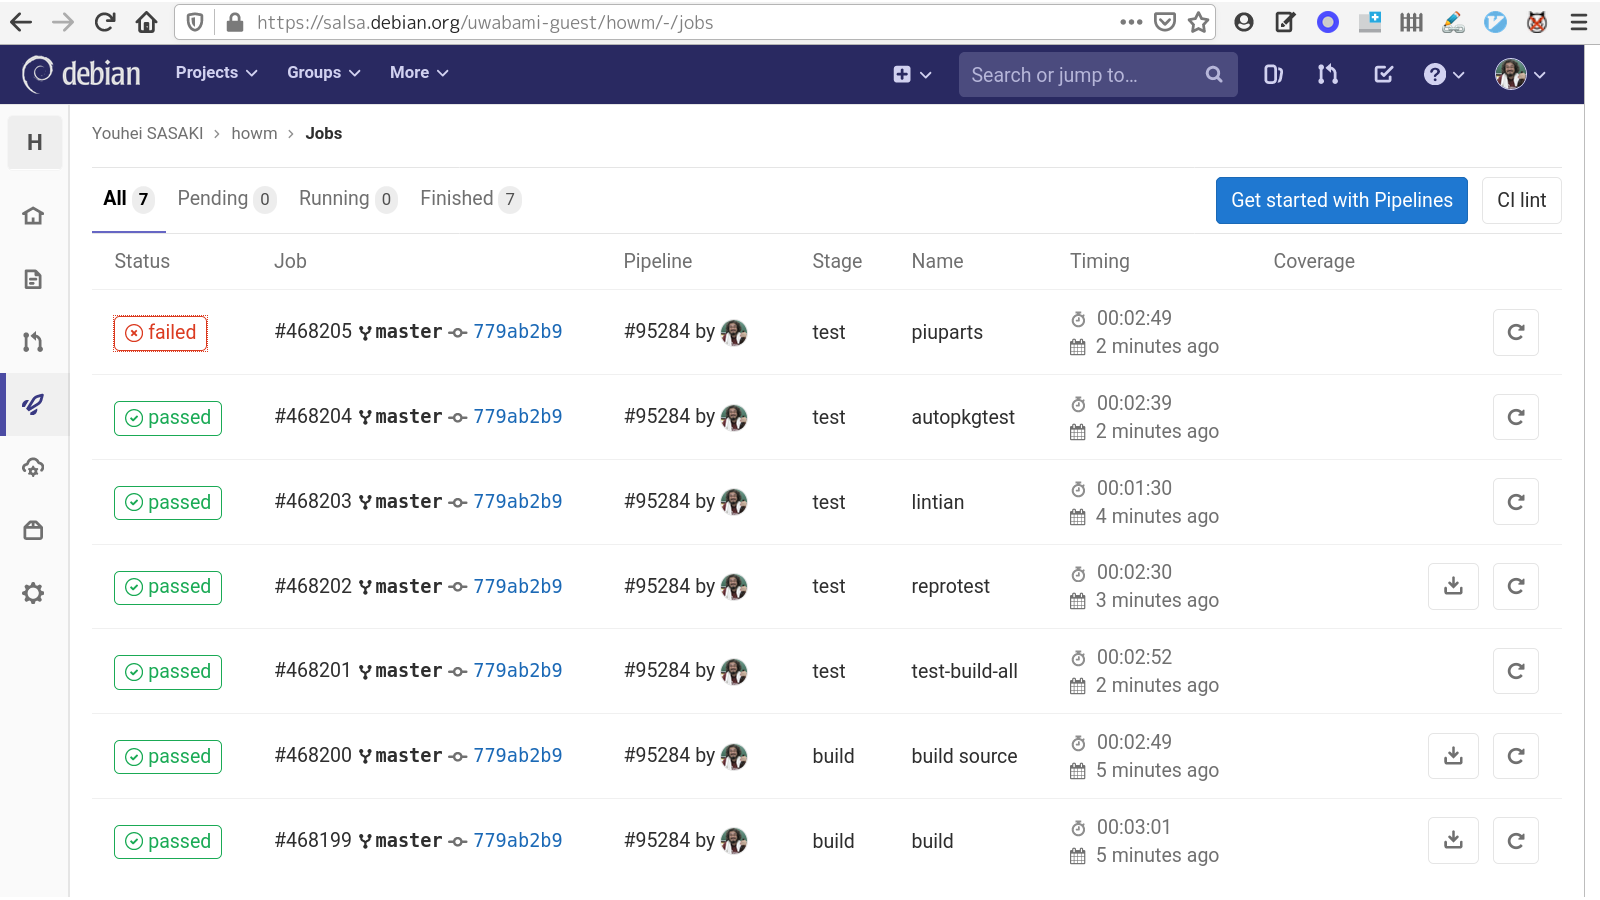
\includegraphics[height=.26\textheight]{image201912/2019-12-22-salsa-ci.png}
  \caption{salsa$B$G$N(BCI$B$N7k2L(B($B$*$d(B, $B0lHV>e$N(Bpipeline$B$NMM;R$,(B...)}
\end{figure}

$B8=>l$+$i$O0J>e$G$9!#(B\hfill($BJY6/2q$4;22C$N3'MM!"$"$j$,$H$&$4$6$$$^$7$?(B)

\clearpage

\dancersection{$B3+:E$NM=Dj(B}{}


\vspace{\fill}
$BK\;qNA$O(B GPL v 2.0 $B$N%i%$%;%s%9$G8x3+$$$?$7$^$9!#(B

\clearpage

%
% $B:};R$K$9$k$?$a$K!"(B4$B$NG\?t$K$9$kI,MW$,$"$k!#(B
% $B$=$N$?$a$ND4@0(B

\mbox{}\newpage
\mbox{}\newpage

\printindex
%\cleartooddpage

 \begin{minipage}[b]{0.2\hsize}
  \rotatebox{90}{\fontsize{80}{80} {\gt $B4X@>(B Debian $BJY6/2q(B} }
 \end{minipage}
 \begin{minipage}[b]{0.8\hsize}

 \vspace*{15cm}
 \rule{\hsize}{1mm}
 \vspace{2mm}
 
\includegraphics[width=2cm,clip]{image200502/openlogo-nd.eps}
 \noindent \Large \bfseries{Debian $BJY6/2q;qNA(B}\\ \\
 \noindent \normalfont \debmtgyear{}$BG/(B\debmtgmonth{}$B7n(B\debmtgdate{}$BF|(B \hspace{5mm}  $B=iHGBh(B1$B:~H/9T(B\\
 \noindent \normalfont $B4X@>(B Debian $BJY6/2q(B $B!JJT=8!&0u:~!&H/9T!K(B\\
 \rule{\hsize}{1mm}
 \end{minipage}

\end{document}
